\documentclass[11pt,a4paper]{article}
\usepackage[T1]{fontenc}
\usepackage[utf8]{inputenc}
\usepackage{lmodern}
\usepackage{textcomp}
\usepackage[left=1.8cm,right=1.8cm,top=2.3cm,bottom=2.2cm,headheight=14pt,headsep=8pt]{geometry}
\usepackage{multicol}
\usepackage{xcolor}
\usepackage{fancyhdr}
\usepackage{graphicx}
\usepackage{array}
\usepackage{amsmath,amssymb}
\usepackage{setspace}
\usepackage{longtable}
\graphicspath{{../}}
\definecolor{ygreen}{RGB}{46,139,87}
\renewcommand{\normalsize}{\fontsize{10.9}{13.4}\selectfont}
\renewcommand{\familydefault}{\rmdefault}
\setlength{\parindent}{0pt}
\setlength{\columnsep}{0.8cm}
\setlength{\columnseprule}{0.4pt}
\setlength{\multicolsep}{3pt plus 1pt minus 1pt}
\renewcommand{\textsubscript}[1]{\ensuremath{_{\text{\fontsize{8}{8}\selectfont #1}}}}
\renewcommand{\textsuperscript}[1]{\ensuremath{^{\text{\fontsize{8}{8}\selectfont #1}}}}
\newcommand{\qn}[1]{\textbf{\fontsize{11.5}{13}\selectfont #1}}
\newcommand{\qsep}{\par\vspace{1pt}\noindent\rule{0pt}{0.4pt}\par\vspace{5pt}}
\newcommand{\fwrule}{\par\vspace{5pt}\noindent\rule{\linewidth}{1.4pt}\par\vspace{7pt}}
\newsavebox{\fitb}
\newcommand{\fitbox}[1]{\sbox{\fitb}{#1}\ifdim\wd\fitb>\linewidth\resizebox{\linewidth}{!}{\usebox{\fitb}}\else\usebox{\fitb}\fi}
\newcommand{\diqqat}[1]{\par\smallskip\noindent\textbf{Diqqat!} #1\par\medskip}
\newcommand{\javob}{\par\smallskip\noindent\textbf{Javob:} \rule[-2pt]{7.5cm}{0.4pt}\par\smallskip\noindent\textbf{Diqqat!} Javobingizni javoblar varaqasiga ko`chirib yozing.\par\medskip}
\pagestyle{fancy}
\fancyhf{}
\renewcommand{\headrulewidth}{0.4pt}
\fancyhead[L]{\textit{Milliy sertifikat 2026. Kimyo}}
\fancyhead[R]{18-variant}
\fancyfoot[L]{\fontsize{8}{9}\selectfont \textcopyright{} Colba maktabi, 2026}
\fancyfoot[C]{\thepage}
\fancypagestyle{first}{\fancyhf{}\renewcommand{\headrulewidth}{0pt}\fancyfoot[L]{\fontsize{8}{9}\selectfont \textcopyright{} Colba maktabi, 2026}\fancyfoot[C]{\thepage}}
\begin{document}
\normalsize
\thispagestyle{first}
\noindent\fcolorbox{ygreen}{white}{\parbox{\dimexpr\linewidth-2\fboxsep-2\fboxrule\relax}{%
\textbf{\fontsize{13}{15}\selectfont Nazorat testi}\ \textit{\fontsize{10}{12}\selectfont $\cdot$ Aralash test $\cdot$ 18-variant}\hfill
\begin{tabular}[t]{@{}r@{}}\textit{Milliy sertifikat 2026. Kimyo}\\ \textbf{\textit{\fontsize{8}{9}\selectfont Vaqt:}} \textit{\fontsize{10}{12}\selectfont 180 daqiqa}\end{tabular}}}
\par\medskip
\noindent\textit{Davriy jadvaldan foydalanish mumkin.}
\par\medskip
\begin{multicols}{2}
\noindent\qn{1.} N\textsubscript{2}O\textsubscript{4} $\rightleftarrows$ 2NO\textsubscript{2} reaksiyasi 1 l hajmli idishda o`tkazildi. Ma'lumotlar jadvalda berilgan:
\begin{center}
\renewcommand{\arraystretch}{1.15}
\fitbox{\begin{tabular}{|c|c|c|}\hline
\textbf{Modda} & \textbf{N\textsubscript{2}O\textsubscript{4}} & \textbf{NO\textsubscript{2}} \\ \hline
Boshlang`ich, mol & 4 & 0 \\ \hline
Muvozanatda, mol & --- & 1 \\ \hline
\end{tabular}}
\end{center}
N\textsubscript{2}O\textsubscript{4} ning necha foizi reaksiyaga \textbf{kirishganini aniqlang.}

\noindent A)~\textsl{12,5} \hfill B)~\textsl{6,2} \hfill C)~\textsl{18,8} \hfill D)~\textsl{87,5}\par
\qsep
\noindent\qn{2.} Rasmda molekulaning sharsimon modeli tasvirlangan (qora -- C, qizil -- O, ko`k -- N, oq -- H).
\begin{center}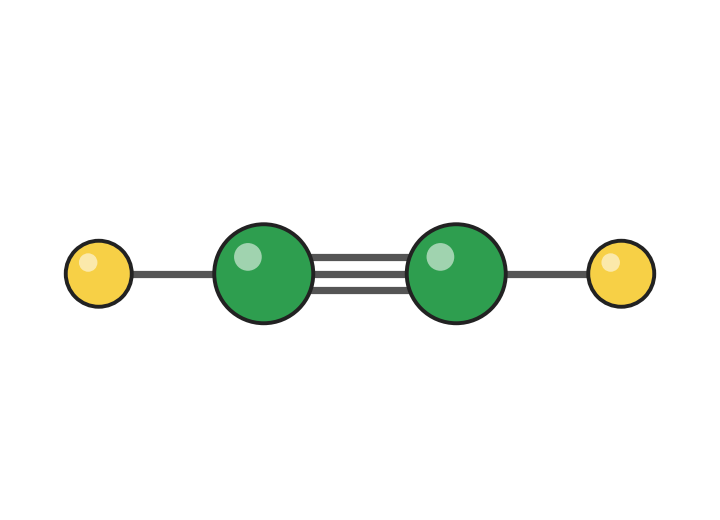
\includegraphics[width=0.86\linewidth]{rasmlar/gen/md_706582.png}\end{center}
Molekula fazoviy shakli qanday?

\noindent\begin{tabular}{@{}p{0.47\linewidth}@{}p{0.47\linewidth}@{}}
A)~\textsl{uchburchakli piramida} & B)~\textsl{burchakli} \\
C)~\textsl{tetraedr} & D)~\textsl{chiziqli} \\
\end{tabular}\par
\qsep
\noindent\qn{3.} H\textsubscript{2}O\textsubscript{2} tarkibida O ning oksidlanish \textbf{darajasini aniqlang.}

\noindent A)~\textsl{$-$2} \hfill B)~\textsl{$-$3 va +5} \hfill C)~\textsl{$-$1} \hfill D)~\textsl{+6}\par
\qsep
\noindent\qn{4.} Na\textsubscript{2}SO\textsubscript{4} eritmasiga 0,5 mol/l li BaCl\textsubscript{2} eritmasi oz-ozdan qo`shilganda hosil bo`lgan cho`kma massasining qo`shilgan hajmga bog`liqligi grafikda keltirilgan.
\begin{center}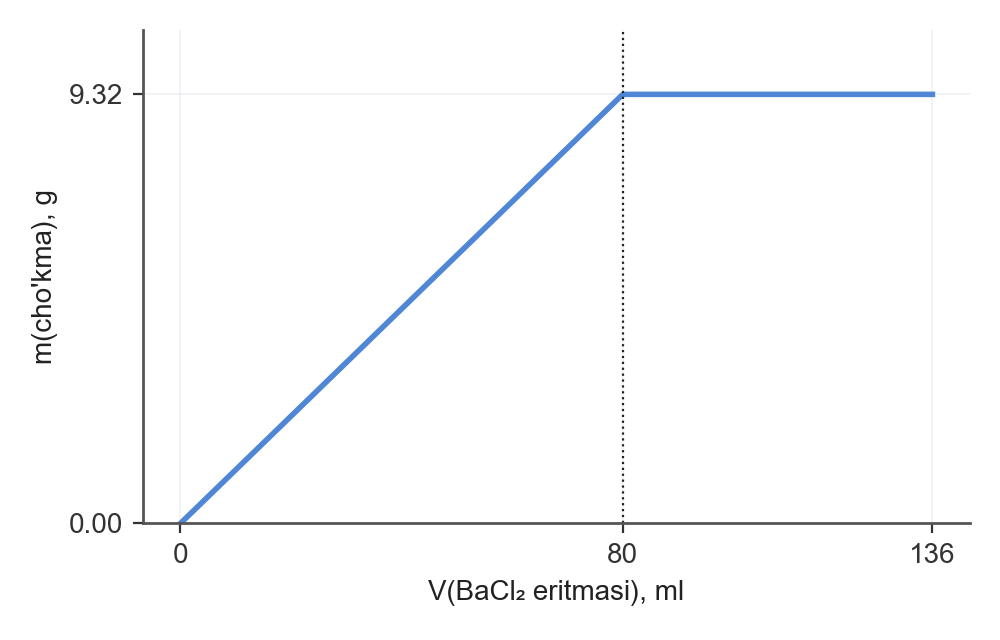
\includegraphics[width=0.86\linewidth]{rasmlar/gen/pp_v18_0.png}\end{center}
Dastlabki eritmadagi Na\textsubscript{2}SO\textsubscript{4} ning \textbf{massasini (g) hisoblang.}

\noindent A)~\textsl{9,32} \hfill B)~\textsl{8,32} \hfill C)~\textsl{5,68} \hfill D)~\textsl{11,36}\par
\qsep
\noindent\qn{5.} 2NO + O\textsubscript{2} $\rightleftarrows$ 2NO\textsubscript{2} reaksiyada muvozanat qaror topganda [NO] = 1, [O\textsubscript{2}] = 1, [NO\textsubscript{2}] = 4 mol/l bo`ldi. NO ning boshlang`ich \textbf{konsentratsiyasini (mol/l) aniqlang.}

\noindent A)~\textsl{5} \hfill B)~\textsl{1} \hfill C)~\textsl{7} \hfill D)~\textsl{3}\par
\qsep
\noindent\qn{6.} Quyidagi jadvalda Na\textsubscript{2}CO\textsubscript{3} tuzining eritmalari keltirilgan:
\begin{center}
\renewcommand{\arraystretch}{1.15}
\fitbox{\begin{tabular}{|c|c|c|}\hline
\textbf{No.} & \textbf{m(eritma), g} & \textbf{$\omega$, \%} \\ \hline
I & 100 & 20 \\ \hline
II & 200 & 30 \\ \hline
\end{tabular}}
\end{center}
Eritmalar aralashtirildi. Oxirgi eritmadagi tuzning massa \textbf{ulushini (\%) toping.}

\noindent A)~\textsl{25} \hfill B)~\textsl{26,67} \hfill C)~\textsl{50} \hfill D)~\textsl{23,33}\par
\qsep
\noindent\qn{7.} 11,2 g Fe va 3,2 g S aralashtirilib, reaksiya o`tkazildi (Fe + S $\to$ FeS). Hosil bo`lgan FeS \textbf{massasini (g) aniqlang.}

\noindent A)~\textsl{17,6} \hfill B)~\textsl{4,4} \hfill C)~\textsl{13,2} \hfill D)~\textsl{8,8}\par
\qsep
\noindent\qn{8.} 8 g NaOH 500 g suvda eritildi. Eritmaning molyal \textbf{konsentratsiyasini (mol/kg) aniqlang.}

\noindent A)~\textsl{0,4} \hfill B)~\textsl{0,39} \hfill C)~\textsl{0} \hfill D)~\textsl{0,8}\par
\qsep
\noindent\qn{9.} Faqat qaytaruvchi bo`la oladigan \textbf{ionlarni aniqlang}: 1) Fe\textsuperscript{3+}; 2) Fe\textsuperscript{2+}; 3) K\textsuperscript{+}; 4) Cl\textsuperscript{$-$}

\noindent A)~\textsl{1} \hfill B)~\textsl{2} \hfill C)~\textsl{1, 3} \hfill D)~\textsl{4}\par
\qsep
\noindent\qn{10.} C\textsubscript{6}H\textsubscript{6} molekulasidagi $\sigma$ va $\pi$ bog`lar \textbf{sonini aniqlang.}

\noindent A)~\textsl{11 va 3} \hfill B)~\textsl{12 va 3} \hfill C)~\textsl{12 va 4} \hfill D)~\textsl{13 va 3}\par
\qsep
\noindent\qn{11.} CH\textsubscript{4} gazining 27 \textdegree{}C va 1 atm bosimdagi \textbf{zichligini (g/l) aniqlang.} (R = 0,082 l$\cdot$atm/(mol$\cdot$K))

\noindent A)~\textsl{1,3} \hfill B)~\textsl{0,33} \hfill C)~\textsl{0,71} \hfill D)~\textsl{0,65}\par
\qsep
\noindent\qn{12.} 3 mol NaCl va 3 mol HNO\textsubscript{3} suvda eritilib, eritma hajmi 4 l ga yetkazildi. Eritmadagi barcha ionlarning umumiy molyar \textbf{konsentratsiyasini (mol/l) aniqlang} (kuchli elektrolitlar to`liq dissotsilanadi).

\noindent A)~\textsl{1,5} \hfill B)~\textsl{6} \hfill C)~\textsl{3} \hfill D)~\textsl{2,25}\par
\qsep
\noindent\qn{13.} Na\textsubscript{2}SO\textsubscript{4} ning suvli eritmasi inert elektrodlar bilan elektroliz qilinganda qaysi moddalar ajraladi?

\noindent A)~\textsl{Ag va O\textsubscript{2}} \hfill B)~\textsl{H\textsubscript{2} va O\textsubscript{2}} \hfill C)~\textsl{Cu va O\textsubscript{2}} \hfill D)~\textsl{Cu va Cl\textsubscript{2}}\par
\qsep
\noindent\qn{14.} Qaysi juftliklar o`zaro reaksiyaga kirishmaydi? 1) Fe\textsubscript{2}O\textsubscript{3} va H\textsubscript{2}O; 2) SiO\textsubscript{2} va H\textsubscript{2}O; 3) Zn va NaOH; 4) NaCl va HNO\textsubscript{3}

\noindent A)~\textsl{3, 4} \hfill B)~\textsl{1, 4} \hfill C)~\textsl{1, 2, 3} \hfill D)~\textsl{1, 2, 4}\par
\qsep
\noindent\qn{15.} Cu + 4HNO\textsubscript{3} $\to$ Cu(NO\textsubscript{3})\textsubscript{2} + 2NO\textsubscript{2} + 2H\textsubscript{2}O jarayoni uchun tarkibida 50\% aralashma bo`lgan 128 g namuna (asosiy modda Cu) olingan. Cu(NO\textsubscript{3})\textsubscript{2} \textbf{massasini (g) aniqlang.}

\noindent A)~\textsl{376} \hfill B)~\textsl{188} \hfill C)~\textsl{94} \hfill D)~\textsl{282}\par
\qsep
\noindent\qn{16.} CO\textsubscript{2} + Ca(OH)\textsubscript{2} $\to$ CaCO\textsubscript{3} + H\textsubscript{2}O reaksiyasida 2,24 l (n.sh.) CO\textsubscript{2} ishtirok etdi. CaCO\textsubscript{3} \textbf{massasini (g) toping.}

\noindent A)~\textsl{20} \hfill B)~\textsl{10} \hfill C)~\textsl{5} \hfill D)~\textsl{15}\par
\qsep
\noindent\qn{17.} NaBr + AgNO\textsubscript{3} $\to$ AgBr + NaNO\textsubscript{3} reaksiyasida tarkibida 60\% aralashma bo`lgan 103 g namuna (asosiy modda NaBr) ishtirok etdi. AgBr \textbf{massasini (g) toping.}

\noindent A)~\textsl{75,2} \hfill B)~\textsl{150,4} \hfill C)~\textsl{37,6} \hfill D)~\textsl{112,8}\par
\qsep
\noindent\qn{18.} Ishqoriy metallar haqida qaysi fikrlar to`g`ri? 1) Kaliy suvdan og`ir; 2) KOH -- kuchli ishqor; 3) Ishqoriy metallar faqat oksidlovchi bo`ladi; 4) Natriy suv bilan reaksiyada H\textsubscript{2} va NaOH hosil qiladi

\noindent A)~\textsl{2, 3} \hfill B)~\textsl{1} \hfill C)~\textsl{1, 2, 4} \hfill D)~\textsl{2, 4}\par
\qsep
\noindent\qn{19.} Alyuminiy va temir dan iborat 13,9 g aralashma mo`l NaOH eritmasida eritildi. Ajralgan gazning \textbf{hajmini (l, n.sh.) aniqlang} (temir ishqor bilan reaksiyaga kirishmaydi).

\noindent A)~\textsl{6,72} \hfill B)~\textsl{3,36} \hfill C)~\textsl{1,68} \hfill D)~\textsl{11,53}\par
\qsep
\noindent\qn{20.} C\textsubscript{5}H\textsubscript{10}O aldegidlarning izomerlari soni nechta?

\noindent A)~\textsl{5} \hfill B)~\textsl{3} \hfill C)~\textsl{4} \hfill D)~\textsl{6}\par
\qsep
\noindent\qn{21.} CH\textsubscript{3}--CH(CH\textsubscript{3})--COOH birikmaning sistematik nomi qaysi qatorda to`g`ri keltirilgan?

\noindent\begin{tabular}{@{}p{0.47\linewidth}@{}p{0.47\linewidth}@{}}
A)~\textsl{butan kislota} & B)~\textsl{3-metilpropan kislota} \\
C)~\textsl{2-metilpropan kislota} & D)~\textsl{2-metilbutan kislota} \\
\end{tabular}\par
\qsep
\noindent\qn{22.} 6,4 g CaC\textsubscript{2} dan quyidagi ikki bosqichda C\textsubscript{2}H\textsubscript{2}Br\textsubscript{4} olinadi: 1) CaC\textsubscript{2} + 2H\textsubscript{2}O $\to$ C\textsubscript{2}H\textsubscript{2} + Ca(OH)\textsubscript{2} (unum 75\%); 2) C\textsubscript{2}H\textsubscript{2} + 2Br\textsubscript{2} $\to$ C\textsubscript{2}H\textsubscript{2}Br\textsubscript{4} (unum 80\%). Oxirgi mahsulot C\textsubscript{2}H\textsubscript{2}Br\textsubscript{4} ning \textbf{massasini (g) toping.}

\noindent A)~\textsl{20,76} \hfill B)~\textsl{27,68} \hfill C)~\textsl{25,95} \hfill D)~\textsl{34,6}\par
\qsep
\noindent\qn{23.} C\textsubscript{2}H\textsubscript{5}OH va CH\textsubscript{3}OH dan iborat 11 g aralashma natriy bilan to`liq reaksiyaga kirishganda ajraladigan vodorod \textbf{hajmini (l, n.sh.) toping.}

\noindent A)~\textsl{3,36} \hfill B)~\textsl{6,72} \hfill C)~\textsl{1,68} \hfill D)~\textsl{1,58}\par
\qsep
\noindent\qn{24.} Aldegid va ketonlar haqida qaysi fikrlar to`g`ri? 1) Sirka aldegid Kucherov reaksiyasi bilan olinadi; 2) Formalin --- formaldegidning 40\% li eritmasi; 3) Aseton Cu(OH)\textsubscript{2} ni qaytaradi; 4) Aseton suvda erimaydi

\noindent A)~\textsl{2, 3, 4} \hfill B)~\textsl{3, 4} \hfill C)~\textsl{1, 2} \hfill D)~\textsl{2, 4}\par
\qsep
\noindent\qn{25.} Karbon kislotalar haqida qaysi fikrlar to`g`ri? 1) Qattiq suvda sovun yaxshi ko`piklanadi; 2) Karboksil guruh karbonil va gidroksil guruhlardan iborat; 3) Olein kislota Br\textsubscript{2} ni biriktiradi; 4) Chumoli kislota "kumush ko`zgu" reaksiyasini beradi

\noindent A)~\textsl{1, 4} \hfill B)~\textsl{1, 2, 4} \hfill C)~\textsl{2, 3, 4} \hfill D)~\textsl{1, 3, 4}\par
\qsep
\noindent\qn{26.} 445 g tristearin gidrolizlanganda necha gramm glitserin hosil bo`ladi?

\noindent A)~\textsl{138} \hfill B)~\textsl{46} \hfill C)~\textsl{23} \hfill D)~\textsl{445}\par
\qsep
\noindent\qn{27.} 68,4 g C\textsubscript{12}H\textsubscript{22}O\textsubscript{11} dan quyidagi ikki bosqichda C\textsubscript{2}H\textsubscript{5}OH olinadi: 1) C\textsubscript{12}H\textsubscript{22}O\textsubscript{11} + H\textsubscript{2}O $\to$ 2C\textsubscript{6}H\textsubscript{12}O\textsubscript{6} (unum 60\%); 2) C\textsubscript{6}H\textsubscript{12}O\textsubscript{6} $\to$ 2C\textsubscript{2}H\textsubscript{5}OH + 2CO\textsubscript{2} (unum 75\%). Oxirgi mahsulot C\textsubscript{2}H\textsubscript{5}OH ning \textbf{massasini (g) toping.}

\noindent A)~\textsl{27,6} \hfill B)~\textsl{22,08} \hfill C)~\textsl{16,56} \hfill D)~\textsl{36,8}\par
\qsep
\noindent\qn{28.} Aminlar, aminokislotalar va oqsillar haqida qaysi fikrlar to`g`ri? 1) Dipeptidda 2 ta peptid bog` bor; 2) Glitsin optik faol; 3) Oqsillar biuret reaksiyasini beradi; 4) Aminokislotalar amfoter birikmalar

\noindent A)~\textsl{1, 4} \hfill B)~\textsl{1} \hfill C)~\textsl{2} \hfill D)~\textsl{3, 4}\par
\qsep
\noindent\qn{29.} 5,2 g C\textsubscript{2}H\textsubscript{2} dan quyidagi ikki bosqichda C\textsubscript{2}H\textsubscript{5}Cl olinadi: 1) C\textsubscript{2}H\textsubscript{2} + H\textsubscript{2} $\to$ C\textsubscript{2}H\textsubscript{4} (unum 80\%); 2) C\textsubscript{2}H\textsubscript{4} + HCl $\to$ C\textsubscript{2}H\textsubscript{5}Cl (unum 75\%). Oxirgi mahsulot C\textsubscript{2}H\textsubscript{5}Cl ning \textbf{massasini (g) toping.}

\noindent A)~\textsl{7,74} \hfill B)~\textsl{9,67} \hfill C)~\textsl{10,32} \hfill D)~\textsl{12,9}\par
\qsep
\noindent\qn{30.} Lakmus indikatori kislotali muhitda qanday rang beradi?

\noindent A)~\textsl{sariq} \hfill B)~\textsl{qizil} \hfill C)~\textsl{binafsha} \hfill D)~\textsl{rangsiz}\par
\qsep
\noindent\qn{31.} Rasmda ammiakning suvda erishi ko`rsatilgan. 22,4 l (n.sh.) NH\textsubscript{3} 1000 g suvda eritilsa, eritmadagi ammiakning massa ulushi necha foiz?
\begin{center}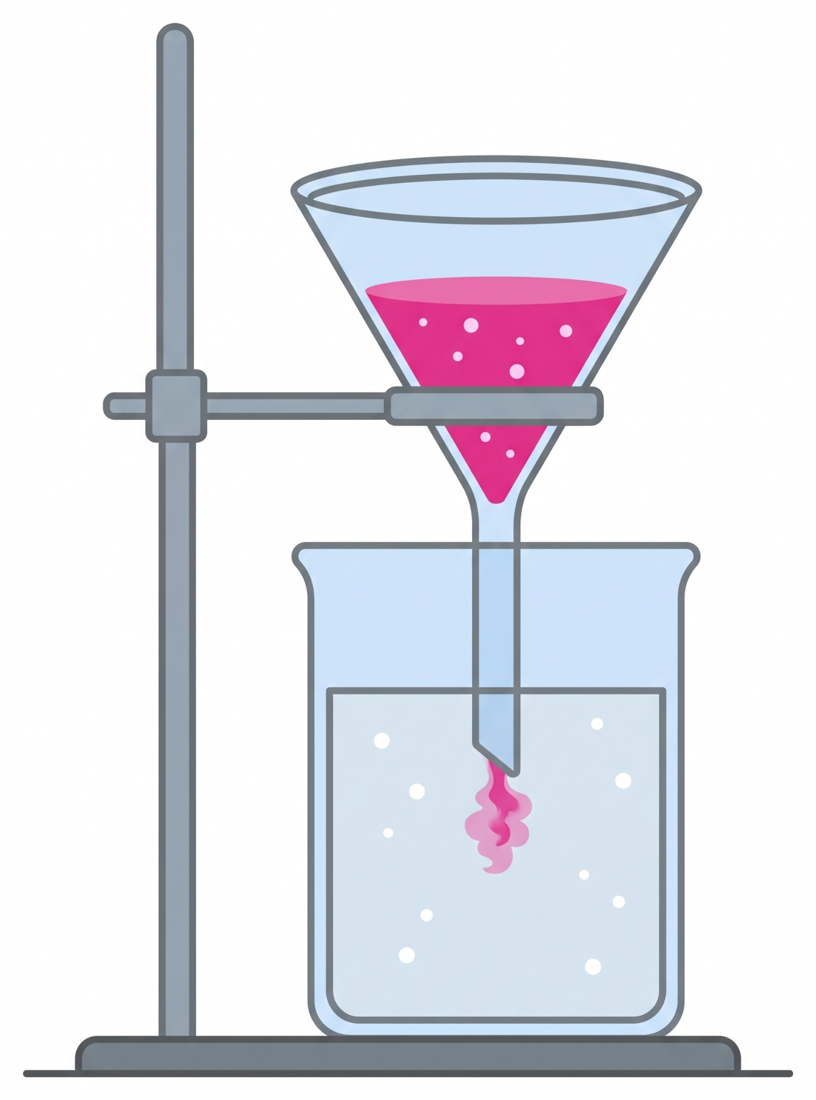
\includegraphics[width=0.86\linewidth]{rasmlar/darslik/d_nh3_fontan.png}\end{center}

\noindent A)~\textsl{1,67} \hfill B)~\textsl{1,7} \hfill C)~\textsl{3,34} \hfill D)~\textsl{0,84}\par
\qsep
\noindent\qn{32.} Kimyo laboratoriyasida ishlash qoidalari haqida qaysi fikrlar to`g`ri? 1) Konsentrlangan kislotani suvga ohista, aralashtirib quyiladi; 2) Kuygan joy ko`p suv bilan yuviladi; 3) Spirt lampa boshqa lampadan yoqilmaydi; 4) Zaharli gaz ajraladigan tajriba mo`rili shkafda o`tkaziladi

\noindent\begin{tabular}{@{}p{0.47\linewidth}@{}p{0.47\linewidth}@{}}
A)~\textsl{1, 2, 4} & B)~\textsl{2, 3, 4} \\
C)~\textsl{1, 2, 3} & D)~\textsl{1, 2, 3, 4   ---} \\
\end{tabular}\par
\qsep
\end{multicols}
\medskip
\noindent\setlength{\fboxsep}{0pt}\fbox{\begin{tabular}{p{0.74\linewidth}|p{0.2\linewidth}}
\parbox[t]{0.72\linewidth}{\vspace{3pt}\textbf{Topshiriqlar (33--35) va javob variant (A--F)larini o`zaro to`g`ri moslashtiring.} CuO va Fe\textsubscript{2}O\textsubscript{3} dan iborat 12 g aralashma qizdirilib, CO oqimida to`liq qaytarildi; qoldiq (metallar) massasi 8,8 g.
\vspace{3pt}} & \parbox[t]{0.19\linewidth}{\vspace{3pt}A~\textsl{2}\\[3pt]
B~\textsl{8,8}\\[3pt]
C~\textsl{8,06}\\[3pt]
D~\textsl{5,38}\\[3pt]
E~\textsl{4}\\[3pt]
F~\textsl{3,2}}\\ \hline
\parbox[t]{0.72\linewidth}{\vspace{2pt}\textbf{33. Aralashmadagi CuO massasini (g) aniqlang.}\vspace{2pt}} & \\ \hline
\parbox[t]{0.72\linewidth}{\vspace{2pt}\textbf{34. Qaytarish uchun (20\% ortiqcha olingan) sarflangan CO hajmini (l, n.sh.) aniqlang.}\vspace{2pt}} & \\ \hline
\parbox[t]{0.72\linewidth}{\vspace{2pt}\textbf{35. Qaytarish natijasida hosil bo`lgan CO\textsubscript{2} massasini (g) aniqlang.}\vspace{2pt}} & 
\end{tabular}}
\par\bigskip
\noindent\qn{36.} Fe + H\textsubscript{2}SO\textsubscript{4} $\to$ Fe\textsubscript{2}(SO\textsubscript{4})\textsubscript{3} + SO\textsubscript{2} + H\textsubscript{2}O reaksiya tenglamasini tenglang. Reagentlar (chap qism) koeffitsiyentlari \textbf{yig`indisini toping.}
\javob\qsep
\noindent\qn{37.} 4 l hajmli yopiq idishda 1 mol N\textsubscript{2}O\textsubscript{4} qizdirilganda N\textsubscript{2}O\textsubscript{4} $\rightleftarrows$ 2NO\textsubscript{2} muvozanati qaror topdi. Muvozanat aralashmasining vodorodga nisbatan zichligi 38,33 ga teng. Shu haroratdagi muvozanat \textbf{konstantasini (K, mol/l) hisoblang.}
\javob\qsep
\noindent\qn{38.} CaCO\textsubscript{3} va MgCO\textsubscript{3} dan iborat 18,4 g aralashma doimiy massagacha qizdirilganda qoldiq massasi 9,6 g bo`ldi. Aralashmadagi CaCO\textsubscript{3} ning \textbf{massasini (g) toping.}
\javob\qsep
\noindent\qn{39.} CH\textsubscript{3}OH va C\textsubscript{2}H\textsubscript{5}OH dan iborat 15,6 g aralashma natriy bilan to`liq reaksiyaga kirishganda ajraladigan vodorod \textbf{hajmini (l, n.sh.) toping.}
\javob\qsep
\noindent\qn{40.} 5,2 g asetilendan Kucherov reaksiyasi bilan (80\% unum) sirka aldegid olindi. Aldegid \textbf{massasini (g) aniqlang.}
\javob\qsep
\par\bigskip\begin{center}\textbf{\fontsize{13}{15}\selectfont YOZMA ISH}\end{center}
\noindent\qn{41.} \textbf{Topshiriqni bajarish jarayonida barcha reaksiya tenglamalarini yozing. Miqdoriy va arifmetik hisoblashlarni (unga asos bo`lgan usul yoki formulani ko`rsatgan holda) uzviy ketma-ketlikda bajaring.}\par\smallskip
Quyidagi eritmalar berilgan: HCl ning 0,02 mol/l li eritmasi va KOH ning 0,04 mol/l li eritmasi. Ularni aralashtirib, umumiy hajmi 1 l bo`lgan eritma tayyorlandi (0,5 l HCl eritmasi va 0,5 l KOH eritmasi). Shuningdek, sirka kislotaning 0,05 mol/l li eritmasida dissotsilanish darajasi 1\%.\par
\noindent 1)Aralashtirilgandan keyingi eritmaning pH ini aniqlang.\par
\noindent 2)Dastlabki HCl eritmasining pH ini hisoblang. 1 l shu eritmadagi HCl massasini (g) ham hisoblang.\par
\noindent 3)Dastlabki KOH eritmasining pH ini hisoblang.\par
\noindent 4)Sirka kislota eritmasidagi H\textsuperscript{+} ionlari konsentratsiyasini (mol/l) va pH ni aniqlang (lg 2 = 0,3, lg 5 = 0,7 ni ishlating). Shuningdek KOH eritmasi 100 marta suyultirilsa pH qancha bo`ladi?\par
\noindent 5)Sirka kislotaning dissotsilanish konstantasini hisoblang (K = C$\alpha$\textsuperscript{2}/(1 $-$ $\alpha$)). Shuningdek HCl eritmasi 10 marta suyultirilsa pH necha bo`ladi?\par
\diqqat{Mazkur topshiriq kengaytirilgan javobni talab etib, uning yechilish usuli va shu usul asosidagi barcha hisoblash amallari javoblar varaqasida aks etishi lozim.}\qsep
\noindent\qn{42.} Reaksiya tenglamalarini tugallang va tenglang. Hosil bo`lgan organik moddalarning tuzilish formulalarini yozing va ularni nomlang.\par
\noindent 1)3C\textsubscript{2}H\textsubscript{2} $\xrightarrow{\text{C, t}}$\par
\noindent 2)CH\textsubscript{3}COONa + NaOH $\xrightarrow{\text{t}}$\par
\noindent 3)CH\textsubscript{2}=CH\textsubscript{2} + Br\textsubscript{2} $\to$\par
\noindent 4)CH\textsubscript{3}--C$\equiv$CH + H\textsubscript{2}O $\xrightarrow{\text{Hg\textsuperscript{2+}}}$\par
\noindent 5)CH\textsubscript{3}COOH + NaHCO\textsubscript{3} $\to$\par
\noindent 6)CH\textsubscript{3}--CH=CH\textsubscript{2} + HBr $\to$\par
\noindent 7)n CH\textsubscript{2}=CH--CH=CH\textsubscript{2} $\to$\par
\diqqat{Mazkur topshiriq kengaytirilgan javobni talab etib, uning yechilish usuli va shu usul asosidagi barcha hisoblash amallari javoblar varaqasida aks etishi lozim.}\qsep
\noindent\qn{43.} \textbf{Topshiriqni bajarish jarayonida barcha reaksiya tenglamalarini yozing. Miqdoriy va arifmetik hisoblashlarni (unga asos bo`lgan usul yoki formulani ko`rsatgan holda) uzviy ketma-ketlikda bajaring.}\par\smallskip
Temir (Fe) va rux (Zn) dan iborat 30,7 g qotishma mo`l suyultirilgan sulfat kislotada eritildi, bunda 11,2 l (n.sh.) gaz ajraldi. Hosil bo`lgan eritmaga mo`l NaOH eritmasi qo`shildi, hosil bo`lgan cho`kma ajratib olindi va havoda qizdirib quritildi.\par
\noindent 1)Reaksiya tenglamalarini yozing va qotishmadagi har bir metallning massasini (g) aniqlang.\par
\noindent 2)Qotishmadagi Fe ning massa ulushini (\%) hisoblang.\par
\noindent 3)Eritish uchun sarflangan 20\% li H\textsubscript{2}SO\textsubscript{4} eritmasining massasini (g) aniqlang.\par
\noindent 4)Mo`l NaOH qo`shilganda hosil bo`lgan cho`kmaning formulasi va massasini (g) toping (reaksiya tenglamalarini yozing).\par
\noindent 5)Cho`kma havoda to`liq qizdirilganda hosil bo`lgan oksidning massasini (g) hisoblang.\par
\diqqat{Mazkur topshiriq kengaytirilgan javobni talab etib, uning yechilish usuli va shu usul asosidagi barcha hisoblash amallari javoblar varaqasida aks etishi lozim.}\qsep
\newpage
\noindent\textbf{\fontsize{13}{15}\selectfont Nazorat testi}\ \textit{$\cdot$ 18-variant}\hfill \textbf{Javoblar kaliti}\par\smallskip\hrule\smallskip
\textit{Faqat o`qituvchi uchun.}\par\medskip
\noindent\textbf{1--32-savollar}\par\smallskip
\noindent\begin{tabular}{|c|c|c|c|c|c|c|c|c|c|c|c|c|c|c|c|}\hline
\textbf{1} & \textbf{2} & \textbf{3} & \textbf{4} & \textbf{5} & \textbf{6} & \textbf{7} & \textbf{8} & \textbf{9} & \textbf{10} & \textbf{11} & \textbf{12} & \textbf{13} & \textbf{14} & \textbf{15} & \textbf{16}\\\hline
\textsl{A} & \textsl{D} & \textsl{C} & \textsl{C} & \textsl{A} & \textsl{B} & \textsl{D} & \textsl{A} & \textsl{D} & \textsl{B} & \textsl{D} & \textsl{C} & \textsl{B} & \textsl{D} & \textsl{B} & \textsl{B}\\\hline
\textbf{17} & \textbf{18} & \textbf{19} & \textbf{20} & \textbf{21} & \textbf{22} & \textbf{23} & \textbf{24} & \textbf{25} & \textbf{26} & \textbf{27} & \textbf{28} & \textbf{29} & \textbf{30} & \textbf{31} & \textbf{32}\\\hline
\textsl{A} & \textsl{D} & \textsl{B} & \textsl{C} & \textsl{C} & \textsl{A} & \textsl{A} & \textsl{C} & \textsl{C} & \textsl{B} & \textsl{C} & \textsl{D} & \textsl{A} & \textsl{B} & \textsl{A} & \textsl{D}\\\hline
\end{tabular}\par\medskip
\noindent\textbf{33--35-savollar}\par\smallskip
\noindent\begin{tabular}{|c|c|c|}\hline \textbf{No} & \textbf{Javob} & \textbf{Qiymat}\\\hline
33 & \textsl{E} & 4\\\hline
34 & \textsl{D} & 5,38\\\hline
35 & \textsl{B} & 8,8\\\hline
\end{tabular}\par\medskip
\noindent\textbf{36--40-savollar}\par\smallskip
\noindent\begin{tabular}{|c|c|}\hline \textbf{No} & \textbf{To`g`ri javob}\\\hline
36 & 8\\\hline
37 & 0,05\\\hline
38 & 10\\\hline
39 & 4,48\\\hline
40 & 7,04\\\hline
\end{tabular}\par\medskip
\noindent\textbf{41--43-topshiriqlar: javoblar}\par\smallskip
\noindent\textbf{41-topshiriq.}\par
\noindent 1) pH = 12\par
\noindent 2) pH = 1,7; 0,73 g\par
\noindent 3) pH = 12,6\par
\noindent 4) pH = 3,3; 10,6\par
\noindent 5) 5,05$\cdot$10\textsuperscript{$-$}6; pH = 2,7\par
\noindent\textbf{42-topshiriq.}\par
\noindent 1) 3C\textsubscript{2}H\textsubscript{2} $\xrightarrow{\text{C, t}}$ C\textsubscript{6}H\textsubscript{6} --- benzol (3 ball)\par
\noindent 2) CH\textsubscript{3}COONa + NaOH $\xrightarrow{\text{t}}$ CH\textsubscript{4} + Na\textsubscript{2}CO\textsubscript{3} --- metan (4 ball)\par
\noindent 3) CH\textsubscript{2}=CH\textsubscript{2} + Br\textsubscript{2} $\to$ CH\textsubscript{2}Br--CH\textsubscript{2}Br --- 1,2-dibrometan (4 ball)\par
\noindent 4) CH\textsubscript{3}--C$\equiv$CH + H\textsubscript{2}O $\xrightarrow{\text{Hg\textsuperscript{2+}}}$ CH\textsubscript{3}COCH\textsubscript{3} --- propanon (aseton) (4 ball)\par
\noindent 5) CH\textsubscript{3}COOH + NaHCO\textsubscript{3} $\to$ CH\textsubscript{3}COONa + H\textsubscript{2}O + CO\textsubscript{2} --- natriy atsetat (3 ball)\par
\noindent 6) CH\textsubscript{3}--CH=CH\textsubscript{2} + HBr $\to$ CH\textsubscript{3}--CHBr--CH\textsubscript{3} --- 2-brompropan (Markovnikov) (3 ball)\par
\noindent 7) n CH\textsubscript{2}=CH--CH=CH\textsubscript{2} $\to$ (--CH\textsubscript{2}--CH=CH--CH\textsubscript{2}--)n --- polibutadiyen (4 ball)\par
\noindent\textbf{43-topshiriq.}\par
\noindent 1) 11,2 g; 19,5 g\par
\noindent 2) 36,5\%\par
\noindent 3) 245 g\par
\noindent 4) 18 g\par
\noindent 5) 16 g\par
\par\bigskip\noindent\textbf{Mavzular taqsimoti}\par\smallskip
{\small\noindent\begin{longtable}{|c|p{7.2cm}|p{5.4cm}|c|}\hline \textbf{No} & \textbf{Mavzu} & \textbf{Tekshiriladigan ko`nikma} & \textbf{Ball}\\\hline
1 & Tirkashev VI bob (muvozanat, jadval) & Jadval tahlili & 1\\\hline
2 & 11-sinf (molekulalar geometriyasi) & Rasm bo`yicha tahlil & 1\\\hline
3 & 8-sinf; Tirkashev \textit{V} bob (oksidlanish darajasi) & Bilim va tushunish & 1\\\hline
4 & Tirkashev \textit{V} bob (almashinish reaksiyalari, grafik) & Grafik tahlili & 1\\\hline
5 & Tirkashev VI bob & Hisoblash va masala yechish & 1\\\hline
6 & Tirkashev III bob (eritmalar, jadval) & Jadval tahlili & 1\\\hline
7 & 8-sinf (ortiqcha modda masalasi) & Hisoblash va masala yechish & 1\\\hline
8 & 11-sinf 4-bob (molyal konsentratsiya) & Hisoblash va masala yechish & 1\\\hline
9 & Tirkashev \textit{V} bob; 11-sinf 7-bob & Bilim va tushunish & 1\\\hline
10 & 10-sinf \S{}17 (gibridlanish); Abdusamatov & Bilim va tushunish & 1\\\hline
11 & 11-sinf (Mendeleyev--Klapeyron) & Hisoblash va masala yechish & 1\\\hline
12 & Tirkashev IV bob (kuchli elektrolitlar) & Hisoblash va masala yechish & 1\\\hline
13 & 11-sinf 8-bob; Tirkashev \textit{V} bob (elektroliz) & Bilim va tushunish & 1\\\hline
14 & 9-sinf; Tashev (anorganik birikmalar xossalari) & Bilim va tushunish & 1\\\hline
15 & 9-sinf; Tirkashev (N/NH\textsubscript{3}/HNO\textsubscript{3}, hisob) & Hisoblash va masala yechish & 1\\\hline
16 & 9-sinf; Tirkashev (P/C/Si, hisob) & Hisoblash va masala yechish & 1\\\hline
17 & 9-sinf; Tirkashev (galogenlar, hisob) & Hisoblash va masala yechish & 1\\\hline
18 & 9-sinf (ishqoriy metallar); Tashev & Bilim va tushunish & 1\\\hline
19 & 9-sinf (alyuminiy) & Hisoblash va masala yechish & 1\\\hline
20 & 10-sinf \S{}6, \S{}12, \S{}20, \S{}28 (izomeriya) & Bilim va tushunish & 1\\\hline
21 & 10-sinf (nomenklatura \S{}6, \S{}11, \S{}20, \S{}24--26) & Bilim va tushunish & 1\\\hline
22 & 10-sinf (ikki bosqichli hisob) & Hisoblash va masala yechish & 1\\\hline
23 & 10-sinf \S{}21 (spirtlar) & Hisoblash va masala yechish & 1\\\hline
24 & 10-sinf (mavzuga oid paragraflar); Abdusamatov & Bilim va tushunish & 1\\\hline
25 & 10-sinf (mavzuga oid paragraflar); Abdusamatov & Bilim va tushunish & 1\\\hline
26 & 10-sinf \S{}29 & Hisoblash va masala yechish & 1\\\hline
27 & 10-sinf (ikki bosqichli hisob) & Hisoblash va masala yechish & 1\\\hline
28 & 10-sinf (mavzuga oid paragraflar); Abdusamatov & Bilim va tushunish & 1\\\hline
29 & 10-sinf (ikki bosqichli hisob) & Hisoblash va masala yechish & 1\\\hline
30 & 8-sinf (indikatorlar) & Bilim va tushunish & 1\\\hline
31 & 8-sinf (24-rasm; eritmalar) & Rasm bo`yicha tahlil & 1\\\hline
32 & 7-sinf (xavfsizlik qoidalari); 10-sinf lab. & Bilim va tushunish & 1\\\hline
33--35 & Aralash masala (moslashtirish) & Ko`p bosqichli hisob & 3\\\hline
36--40 & Qisqa javobli masalalar & Hisoblash & 5\\\hline
41--43 & Yozma ish & Usul va hisob (M, A) & 75\\\hline
\end{longtable}}
\end{document}
